\chapter{Zeitenkontrolle}
Für die Zeitenkontrolle wurden die Daten aus Jira ausgewertet und im folgenden Abschnitt analysiert.

\section{Zeitaufwand pro Person }
\begin{figure}[H]
	\centering
	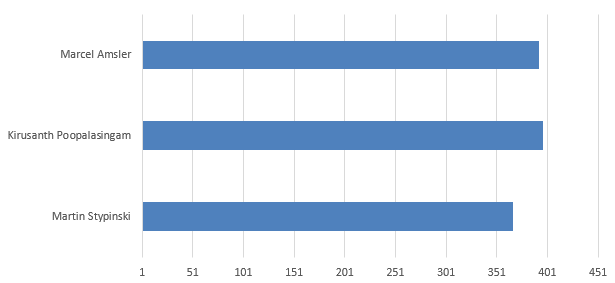
\includegraphics[width=1.0\textwidth] {images/time-per-person.png}
	\caption{Zeitaufwand pro Person in Stunden}
	\label{fig:time}
\end{figure}

Die gezeigte Grafik \ref{fig:time} zeigt total aufgewendeten Stunden während dem Projekt pro Teammitglied. Es wurden deutlich mehr Stunden investiert, als die geforderten 350, welche 12 ECTS Punkten entsprechen. Zurückzuführen ist dies auf gewisse Hüren in der Implementation, welche aus der Risikoanalyse nicht ganz ersichtlich waren. Um das Produkt in unserem Interesse abzuschliessen und ein vollwertige Plattform zu entwickeln, wurde im Kollektiv beschlossen, dass eine Überschreitung im Sinne des Projektes ist.

\section{Zeitaufwand nach Task}
\begin{figure}[H]
	\centering
	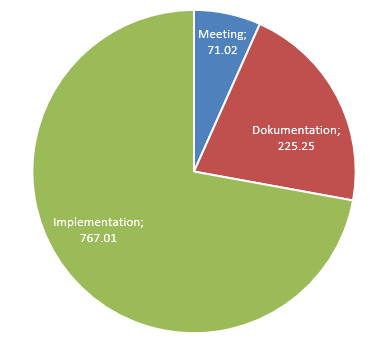
\includegraphics[width=0.6\textwidth] {images/time-per-category.png}
	\caption{Zeitaufwand pro Person in Stunden}
	\label{fig:time-per-category}
\end{figure}

Wie aus der Grafik \ref{fig:time-per-category} zu entnehmen ist, wurde für die Implementierung die meiste Zeit aufgewendet. Da das Testing bei uns zur Implementierung gehört (siehe Kapitel \ref{quality-assurance} Qualitätssicherung ), wird diese Kategorie nicht seperat geführt. Zu den Meetings gehören, neben dem Treffen mit dem Betreuer und der Präsentation, auch jeweils längere interen Diskussion im Team.

